\documentclass[../main.tex]{subfiles}
\graphicspath{{\subfix{../figures/}}}

\begin{document}
\section{实验步骤}
\subsection{攻击准备}
准备硬件和软件:
\begin{itemize}
  \item 硬件:
    \begin{itemize}
      \item PC.
      \item ESP8266 Wi-Fi 模块.
    \end{itemize}
  \item 软件:
    \begin{itemize}
      \item Arduino IDE.
      \item 安信可串口调试助手.
      \item Flash Download Tool.
      \item esp8266\_deauther.
      \item Python-3.
    \end{itemize}
\end{itemize}

下面编译生成需要在 ESP8266 上执行的固件:
\begin{minted}{sh}
git clone https://github.com/SpacehuhnTech/esp8266_deauther
cd esp8266_deauther/esp8266_deauther
python3 ../utils/arduino-cli-compile.py 2.5.0
\end{minted}

编译完成后会得到一个 bin 文件, 需要将这个文件上传至 ESP8266, 需要用到 Flash
Download Tool(需先将 ESP8266 同 PC 连接).

\begin{figure}[H]
  \begin{center}
    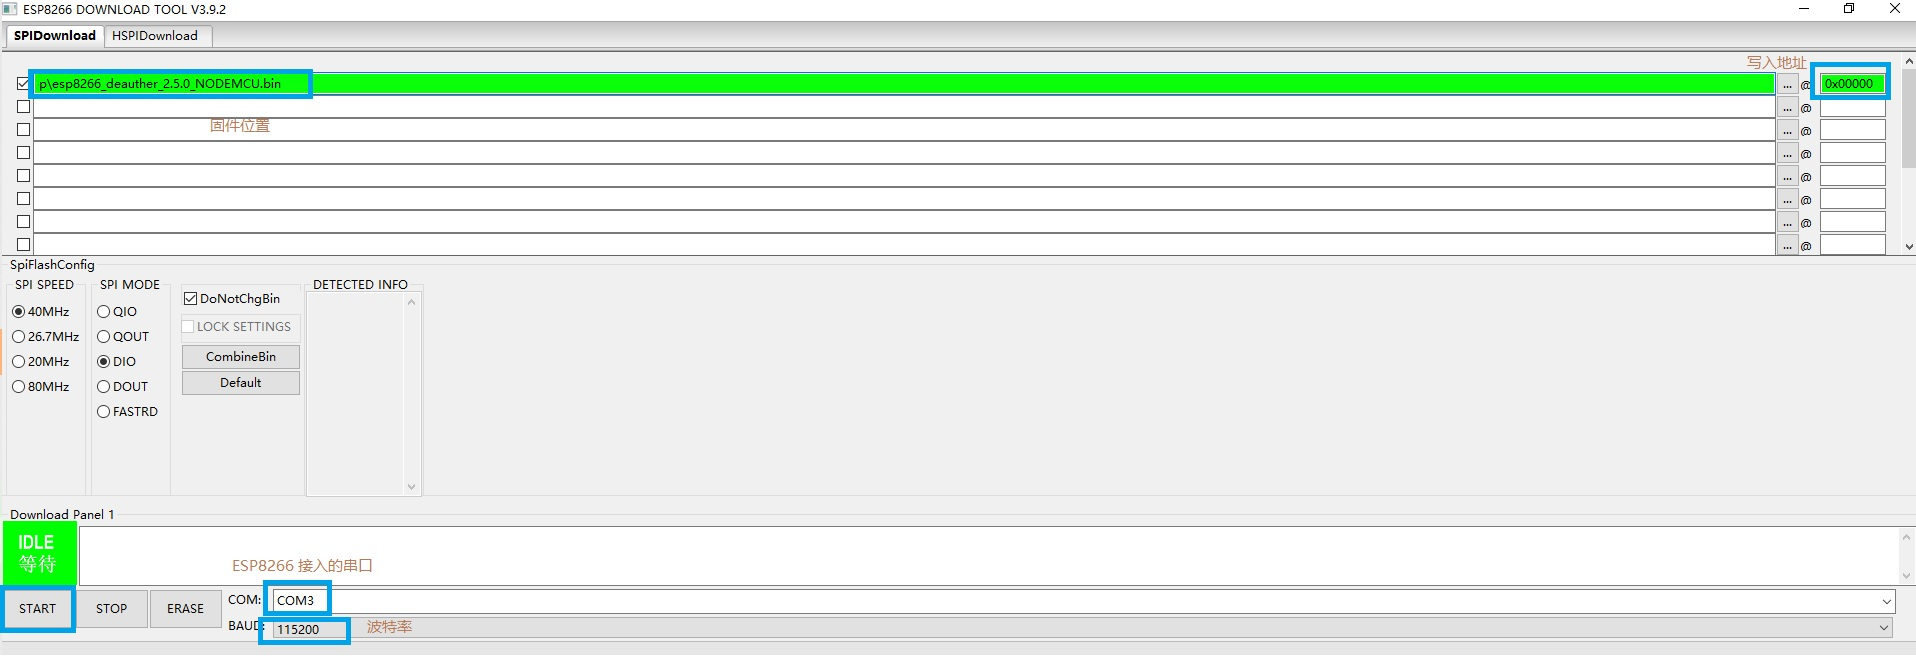
\includegraphics[width=0.30\textwidth]{flash.jpg}
  \end{center}
  \caption{代码烧录}
\end{figure}

设置完毕后点击 ``Start'' 开始烧录.

至此我们完成了环境的设置和代码的上传, 下面就是``指挥'' ESP8266 实施攻击.
%
\subsection{实施攻击}
\subsection{结果分析}
\end{document}
